\documentclass[12pt]{article}

\usepackage[utf8]{inputenc}
\usepackage[T1]{fontenc}
\usepackage{graphicx}
\usepackage{amsmath}
\usepackage[left=0.5in, right=0.5in, top=1in, bottom=1in]{geometry}
\title{\textbf{Banking System Requirement Specification}\\[1cm]
\large Group 15 \\[0.5cm]
{\normalfont YuHang Zhu}}
\author{}
\date{April 13 . 2024}

\begin{document}

\begin{titlepage}
\maketitle
\end{titlepage}

\newpage

\section{Introduction}



\subsection{Purpose}

The objective of the bank system project is to design and develop a comprehensive and efficient banking system that caters to the needs of both account holders and banking facilities. The system encompasses various features such as a database to store all account data, checking and saving accounts, an interface for a mobile application, and an interface specifically designed for ATMs.

\subsection{Scope}

The scope of the bank system project encompasses the following core functionalities:

\begin{enumerate}
\item Database Management: Implementation of a centralized database to store comprehensive account data, including information related to checking and saving accounts. This database will ensure efficient data management and retrieval for account-related transactions.

\item Account Management: Provision of features for managing checking and saving accounts, including the ability to open and close accounts as per customer preferences and requirements.

\item Mobile Application Interface: Development of a user-friendly interface accessible through a mobile application. This interface will enable customers to perform essential banking tasks such as transferring money to other individuals and managing account status.

\item ATM Interface: Integration of an intuitive interface specifically designed for Automated Teller Machines (ATMs). Through this interface, customers will be able to conveniently deposit and withdraw cash, as well as query their account details securely.
\end{enumerate}

\newpage 
\section{Use Case Diagram}
\begin{figure}[h]
    \centering
    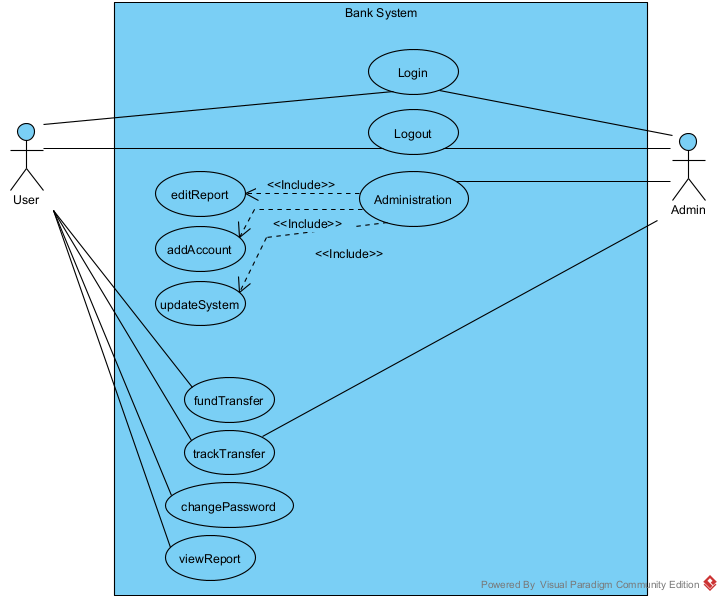
\includegraphics[width=\linewidth]{WeeklyReport/BankSysUseCase.png}
    \caption{Basic use case of banking system }
    \label{fig:usecase}
\end{figure}

As shown in Figure \ref{fig:usecase}, the banking system allows users and admins to log in and out, perform fund transfers, track transfers, change passwords, and view reports. Additionally, admins can perform administrative tasks such as editing reports, adding accounts, and updating system settings.

\newpage
\section{Class Diagram}

\begin{figure}[h]
    \centering
    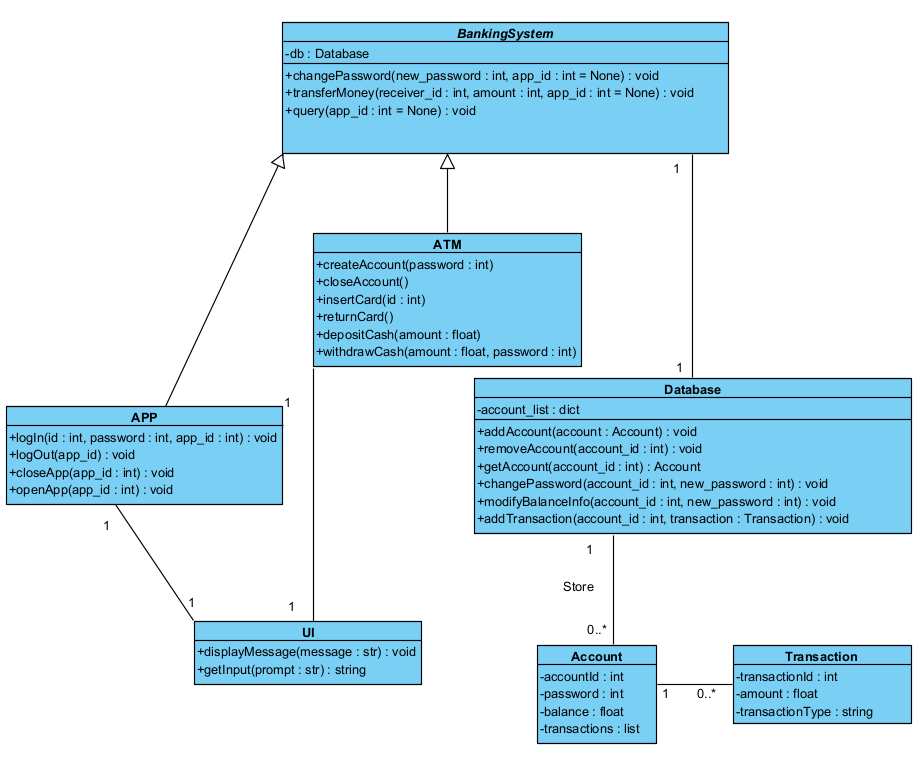
\includegraphics[width=\linewidth]{WeeklyReport/class_diagram.png}
    \caption{Basic class diagram of banking system }
    \label{fig:classdiagram}
\end{figure}

As shown in Figure \ref{fig:classdiagram}, subclasses APP and ATM under BankingSystem are responsible for implementing basic functions, the UI class handles interface presentation and input processing, and the Database class stores accounts and their associated transaction information.
\newpage

\section{Functional Boundaries and Limitations}
\subsection{ATM Functionality}

\begin{enumerate}
    \item \textbf{create\_account@password}
        \begin{itemize}

            \item Constraint1: Account IDs should consist of 10 digits.
            \item Constraint2: No duplicate account IDs or usernames.
            \item Constraint3: Password length and complexity (e.g., Way 1. minimum of 8 characters, including uppercase letters, lowercase letters, and numbers. Way 2. consist of exactly 6 digits).
        \end{itemize}
        
    \item \textbf{close\_account}
        \begin{itemize}
            \item Constraint1: Ensure the account balance is zero before closing the account.
            \item Constraint2*: User identity verification (e.g., through password) should be performed before closing the account. 
            \item Constraint3: The account must not be logged in on the app.
        \end{itemize}
        
    \item \textbf{insert\_card@id}
        \begin{itemize}
            \item Constraint1: Validity and existence of the account IDs.
            \item Constraint2*: Check if the card is blacklisted or frozen.
        \end{itemize}
        
    \item \textbf{return\_card}
        \begin{itemize}
            \item Constraint1*: Check for any unfinished transactions at APP before the card is returned.
            \item Constraint2: Ensure the card has been inserted in ATM before returning.
        \end{itemize}
        
    \item \textbf{deposit\_cash@num}
        \begin{itemize}
            \item Constraint1: Minimum and maximum values for the deposit amount (e.g $ \$0.01\sim \$50000.00$).
            \item Constraint2*: Check if the cash capacity of the ATM is sufficient to store the new cash.
            \item Constraint3*: Check for any unfinished transactions at APP before the card is returned.
            \item Constraint4: Update the database.
        \end{itemize}
        
    \item \textbf{withdraw\_cash@num@password}
        \begin{itemize}
            \item Constraint1: Sufficient account balance for withdrawal.
            \item Constraint2: Password verification.
            \item Constraint3*: Availability of cash inventory in the ATM.
            \item Constraint4*: Check for any unfinished transactions at APP before the card is returned.
            \item Constraint5: Update the database.
        \end{itemize}
\end{enumerate}

\subsection{APP Functionality}

\begin{enumerate}
    \item \textbf{log\_in@id@password\#app\_id}
        \begin{itemize}
            \item Constraint1: Correct format for account ID, password and app ID.
            \item Constraint2: The app to log in is opened.
            \item Constraint3.1*: If login fails, repeatedly request the correct ID and password.
            \item Constraint3.2*: Limit on the number of login attempts (to prevent brute-force attacks), multi-factor authentication.
        \end{itemize}
        
    \item \textbf{log\_out\#app\_id}
        \begin{itemize}
            \item Constraint1: Check if the user is logged in.
            \item Constraint2: Correct format for app ID.
            \item Constraint3*: Ensure all unsaved data is saved before logout.
        \end{itemize}
        
    \item \textbf{close\_app\#app\_id}
        \begin{itemize}
            \item Constraint1: Correct format for app ID.
            \item Constraint2: Check if the application is in use (e.g log out the using account).
            \item Constraint3*: Ensure all unsaved data is saved before closing.
        \end{itemize}
\end{enumerate}

\subsection{Both (Shared Functionality)}

\begin{enumerate}
    \item \textbf{change\_password@new\_password(\#app\_id)}
        \begin{itemize}
            \item Constraint1: Correct format for the new password and app ID.
            \item Constraint2: Avoid using the old password as the new password, multi-factor authentication.
            \item Constraint3: The state of account should be logged in APP or inserted-card in ATM.
            \item Constraint4: Update the database.
        \end{itemize}
        
    \item \textbf{transfer\_money@receiver\_id@num(\#app\_id)}
        \begin{itemize}
            \item Constraint1: Minimum and maximum values for the transfer amount (e.g $ \$0.01\sim \$50000.00$).
            \item Constraint2: Valid state of account and correct format for the app ID and account ID.
            \item Constraint3: Ensure sufficient account balance, validity of the receiver's account, prevent duplicate transfers.
            \item Constraint4: Update the database.
        \end{itemize}
        
    \item \textbf{query(\#app\_id)}
        \begin{itemize}
            \item Constraint1*: Limit on query frequency (to prevent excessive querying).
            \item Constraint2: Valid state of account and correct format for the app ID and account ID.
            \item Constraint3: Get the account's balance, transaction log and *password.
        \end{itemize}
\end{enumerate}

\subsection{other}
\begin{enumerate}
    \item \textbf{open\_app}
        \begin{itemize}
            \item Constraint1: open the ${i+1}_{th}$ APP, where the i is the num of APP opened 
        \end{itemize}
    \item \textbf{reset}
        \begin{itemize}
            \item Constraint1: Only need to delete all the data stored in database.
        \end{itemize}
\end{enumerate}

\subsection{Failure Cases (Errors)}

Consider the following tests when operations above fail:
\begin{itemize}
    \item Provide clear error messages to help users understand the issue.
    \item *Ensure system consistency after the error occurs (e.g., transaction rollback).
    \item *Log all failed attempts for future analysis and improvement.
\end{itemize}
NOTE : (* represents the optimal functional limitation we could consider later.)



\end{document}